\documentclass{article}
\usepackage{tikz}
\usetikzlibrary{trees,shadows}
\begin{document}

\begin{figure}[htbp]
\centering
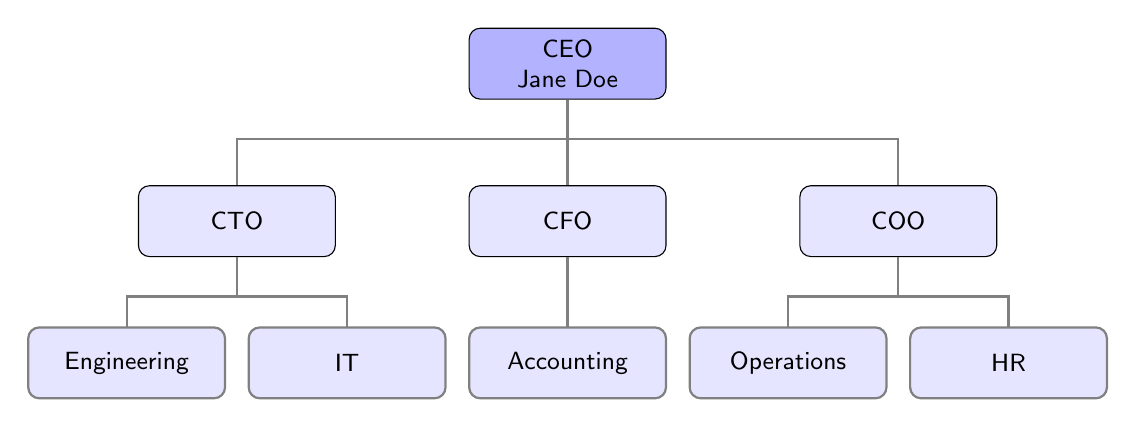
\begin{tikzpicture}[
  every node/.style={draw, fill=blue!10, rounded corners, minimum width=2.5cm, minimum height=0.9cm, align=center, font=\sffamily\small},
  level 1/.style={sibling distance=4.2cm, level distance=2cm},
  level 2/.style={sibling distance=2.8cm, level distance=1.8cm},
  edge from parent/.style={draw, thick, gray},
  edge from parent path={(\tikzparentnode.south) -- +(0,-0.5cm) -| (\tikzchildnode.north)}
]
\node[fill=blue!30] {CEO\\Jane Doe}
  child {node {CTO}
    child {node {Engineering}}
    child {node {IT}}
  }
  child {node {CFO}
    child {node {Accounting}}
  }
  child {node {COO}
    child {node {Operations}}
    child {node {HR}}
  };
\end{tikzpicture}
\caption{Organisation chart.}
\end{figure}

\end{document}
